\documentclass[tikz,border=5pt]{standalone}
\usepackage[UTF8]{ctex}\usepackage{amsmath,amssymb}
\usetikzlibrary{arrows.meta,calc}
\definecolor{ink}{HTML}{243447}\definecolor{blue}{HTML}{2765A2}
\definecolor{green}{HTML}{3F7D5B}\definecolor{red}{HTML}{B74739}
\tikzset{body/.style={draw=ink,thick},vec/.style={draw=blue,thick,-{Latex}},guide/.style={gray!65,dashed},dim/.style={ink,{Latex}-{Latex}},line cap=round,line join=round}
\begin{document}
\begin{tikzpicture}
 \draw[body,fill=blue!5](-1.8,0)arc[start angle=180,end angle=360,x radius=1.8,y radius=.5]
 --(1.8,-.25)arc[start angle=0,end angle=-180,x radius=1.8,y radius=.5]--cycle;
 \draw[body,fill=blue!3](0,0)ellipse(1.8 and .5);
 \fill[ink](0,0)circle(.035);\draw[vec](0,0)--(1.75,.08)node[midway,above]{$r$};
 \draw[body](-.8,.33)--(-.8,1.12);
 \draw[body](-.8,.33)--(-1.02,-.03)(-.8,.33)--(-.58,-.03);
 \draw[body](-.8,.85)--(-1.1,.6)(-.8,.85)--(-.5,.6);
 \draw[body](-.8,1.34)circle(.2);
 \node[above]at(-.8,1.62){$m$};\node[below]at(0,-.9){圆盘质量 $m$};
 \begin{scope}[shift={(5.2,.2)}]
 \draw[body](0,0)circle(1.65);
 \coordinate(A)at(90:1.65);\coordinate(B)at(210:1.65);\coordinate(D)at(330:1.65);
 \draw[vec](A)--(B);\draw[vec](B)--(D);\draw[vec](D)--(A);
 \fill[ink](0,0)circle(.03);\node[below]at(0,0){$O$};
 \node[above]at(A){出发点};
 \node at(0,-2.05){地面路径};
 \end{scope}
\end{tikzpicture}
\begin{tikzpicture}
 \draw[body](0,0)circle(2);
 \draw[guide](0,0)--(0:2);
 \draw[red,thick](0,0)--(-38:2)node[right]{盘面标记};
 \draw[vec](0,0)--(72:2)node[above]{$P$};
 \draw[red,thick,-{Latex}](.7,0)arc[start angle=0,end angle=-38,radius=.7];
 \node[red]at(-19:.95){$\theta$};
 \draw[green,thick,-{Latex}](-38:1.2)arc[start angle=-38,end angle=72,radius=1.2];
 \node[green]at(18:1.48){$\psi$};
 \draw[blue,thick,-{Latex}](1.75,0)arc[start angle=0,end angle=72,radius=1.75];
 \node[blue]at(55:2.1){$\varphi$};
 \fill[ink](0,0)circle(.035);\node[below left]at(0,0){$O$};
 \node at(0,-2.45){$\varphi=\theta+\psi$；角度为有向累计量};
\end{tikzpicture}
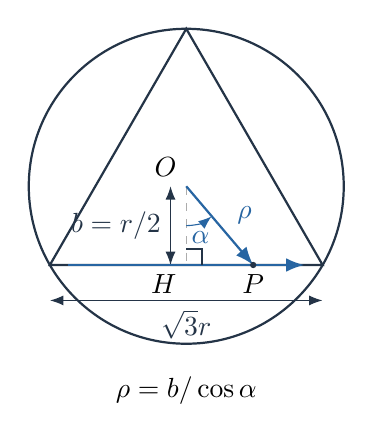
\begin{tikzpicture}
 \draw[body](0,0)circle(2);
 \coordinate(A)at(90:2);\coordinate(B)at(210:2);\coordinate(D)at(330:2);
 \draw[body](A)--(B)--(D)--cycle;
 \coordinate(H)at(0,-1);\coordinate(P)at(.85,-1);
 \draw[guide](0,0)--(H);\draw[vec](0,0)--(P);
 \node[blue]at(.74,-.37){$\rho$};
 \draw[dim](-.2,0)--(-.2,-1)node[midway,left]{$b=r/2$};
 \draw[vec](-1.5,-1)--(1.5,-1);
 \draw[body](0,-.8)--(.2,-.8)--(.2,-1);
 \fill[ink](P)circle(.04);\node[below]at(P){$P$};\node[below left]at(H){$H$};
 \draw[blue,-{Latex}](0,-.5)arc[start angle=-90,end angle=-50,radius=.5];
 \node[blue]at(.18,-.65){$\alpha$};
 \node[above left]at(0,0){$O$};
 \draw[dim](-1.73,-1.45)--(1.73,-1.45)node[midway,below]{$\sqrt3r$};
 \node at(0,-2.6){$\rho=b/\cos\alpha$};
\end{tikzpicture}
\begin{tikzpicture}
 \coordinate(C)at(0,0);\coordinate(P)at(0,1.125);\coordinate(O)at(0,-1.125);
 \draw[body,fill=blue!3](O)circle(2.25);
 \draw[guide](C)circle(1.125);
 \draw[green,thick](90:1.125)--(210:1.125)--(330:1.125)--cycle;
 \draw[body](O)--(P);
 \fill[ink](C)circle(.04);\fill[blue](O)circle(.04);\fill[red](P)circle(.045);
 \node[left]at(C){$C$固定};\node[below left]at(O){$O$移动};
 \node[right]at(P){$P$};
 \draw[dim](1.5,-1.125)--(1.5,1.125)node[midway,right]{$OP=r$（边缘）};
 \draw[vec](0,1.125)--(-.6,.075);
 \draw[vec](0,-1.125)--(.6,-.075);
 \node at(.4,1.65){$CP=CO=OP/2$};
 \node at(0,-3.75){地面边缘圆半径 $r/2$；绿色为闭合地面路径};
\end{tikzpicture}
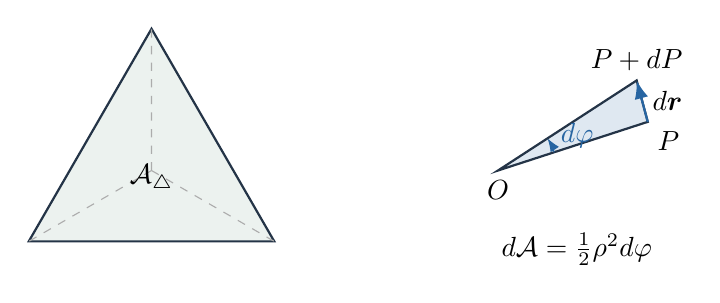
\begin{tikzpicture}
 \coordinate(O)at(0,0);\coordinate(A)at(90:1.8);\coordinate(B)at(210:1.8);\coordinate(D)at(330:1.8);
 \fill[green!10](A)--(B)--(D)--cycle;\draw[body](A)--(B)--(D)--cycle;
 \draw[guide](O)--(A)(O)--(B)(O)--(D);
 \node at(0,-.1){$\mathcal A_\triangle$};
 \begin{scope}[shift={(4.4,0)}]
 \coordinate(P)at(18:2);\coordinate(Q)at(33:2.1);
 \fill[blue!15](0,0)--(P)--(Q)--cycle;
 \draw[body](0,0)--(P)--(Q)--cycle;
 \draw[vec](P)--(Q)node[midway,right]{$d\boldsymbol r$};
 \node[below]at(0,0){$O$};
 \node[below right]at(P){$P$};\node[above]at(Q){$P+dP$};
 \draw[blue,-{Latex}](18:.75)arc[start angle=18,end angle=33,radius=.75];
 \node[blue]at(24:1.1){$d\varphi$};
 \node at(1,-1){$d\mathcal A=\tfrac12\rho^2d\varphi$};
 \end{scope}
\end{tikzpicture}
\end{document}
